\RequirePackage[T1]{fontenc}
\documentclass[acmsmall,screen,nonacm]{acmart}
\usepackage{amsmath,booktabs,tabularx}
\setlength{\emergencystretch}{2em}
\settopmatter{printacmref=false}
\setcopyright{none}
\authorsaddresses{}
\newcolumntype{Y}{>{\raggedright\arraybackslash}X}
\title[When Majority Voting Fails]{When Majority Voting Fails: A Reproducible Study of Citation-Verification Consensus}
\subtitle{Controlled Reanalysis, Source-Held-Out Evaluation, and Corrected-Label Robustness}
\author{Chinmay Thakur}
\affiliation{\institution{Indian Institute of Information Technology Allahabad}\city{Prayagraj}\country{India}}
\renewcommand{\shortauthors}{Chinmay Thakur}
\begin{document}
\begin{abstract}
Combining citation checkers appears to offer a simple way to reduce unreliable alerts, but agreement is not evidence of correctness. This study implements and evaluates hard-voting and review-deferral rules on the released decisions of five citation-verification tools for 104 references from three documents. The original release reproduces the published RefChecker confusion matrix exactly. A subsequent audit identifies an author-corrected release with two changed labels; both versions are retained, and all methods are rerun without changing their decision rules. On the corrected release, majority voting has recall 0.886 and a false-positive rate of 0.522, compared with 0.971 and 0.493 for RefChecker. It fails the prespecified requirement to reduce the false-positive rate by at least 0.10 while retaining recall of at least 0.80. Requiring four votes improves pooled balanced accuracy to 0.792 but reduces recall to 0.714. Threshold selection using only the other source documents yields balanced accuracy 0.704, illustrating the limits of the favorable pooled result. A fixed triage rule defers 53 references and makes nine errors among 51 automatic decisions. The contribution is an auditable implementation and a bounded negative result about consensus on recorded checker decisions, not a new citation verifier or a live benchmark of the underlying tools.
\end{abstract}
\keywords{citation integrity, bibliographic verification, ensemble voting, reproducibility, negative results, selective prediction}
\maketitle
\noindent\textbf{Course:} AI Tools for Research \quad \textbf{Topic:} T23 \quad \textbf{Roll:} MDE2026011\\
\textbf{Programme:} M.Tech (Information Technology), Data Engineering\\
\textbf{Study and verification date:} 18 October 2026

\section{Introduction}
A citation can be well formatted while identifying the wrong work. It can identify a real work while failing to support the surrounding claim. The preceding T23 literature review separated presentation, bibliographic identity, access, and evidential support \citep{thakur2026}. The present implementation study takes one narrow part of that framework: deciding which bibliographic references should be flagged for further checking. It does not experimentally measure formatting quality, reader trust, or whether a source entails a claim.

The motivating practical question is whether several imperfect checkers can provide a better alert policy than one checker. A majority rule is inexpensive and inspectable: count the flags and compare the count with a threshold. However, the rule has no mechanism for finding new bibliographic evidence. If checkers share difficult records or frequently flag legitimate references, agreement can reproduce those mistakes. Conversely, a problem recognized by only one or two tools can disappear under majority voting. These possibilities make the benefit of consensus an empirical question.

This study uses the public reference-level decisions accompanying Badalova and Mayr's evaluation \citep{badalova2026,datasetv1,datasetv11}. The implementation recomputes the five recorded checker baselines, combines their flags, preserves document boundaries for adaptive threshold selection, and exports every prediction. It establishes a reproducible baseline before interpreting the combinations. The resulting experiment is a controlled reanalysis of existing observations with new post-processing, rather than a rerun of the original services. That distinction is central: network retrieval, extraction, and the original tools' runtime are outside the measured system.

The primary hypothesis is deliberately falsifiable. A three-of-five majority must reduce RefChecker's false-positive rate by at least ten percentage points while retaining recall of at least 0.80 on the frozen corpus. This criterion expresses a useful-alert objective, rather than maximizing accuracy after seeing the outcomes. It is not met on either dataset version. The negative result is retained as the main result; a favorable secondary threshold is not substituted for the prespecified rule.

The study contributes an executable consensus and triage module; a validated reconstruction of a published baseline; a comparison of fixed thresholds, source-held-out selection, and panel ablations; and a version-aware audit showing how a small label correction changes evaluation. It claims neither a novel voting algorithm nor general superiority over current citation-verification systems.

\section{From the Review to an Executable Study}
\subsection{Verified methodological context}
CheckIfExist uses a cascade of bibliographic sources, including Crossref, Semantic Scholar, and OpenAlex, with string-based matching \citep{abbonato2026}. Its official repository was accessible and carried an MIT license at the time of inspection. Running its live pipeline would introduce network availability and changing database contents into the experiment. Here, its already-recorded binary decisions provide one comparator.

CiteAudit describes a multi-stage verification framework involving extraction, memory lookup, retrieval, and judgment \citep{shi2026}. Its public repository was accessible, but the inspected workflow required external service credentials. It was therefore considered in the feasibility analysis rather than implemented in this CPU-only study. Public access to a repository was not treated as proof that every dependency or redistribution right was available.

ALCE evaluates citation-supported text generation \citep{gao2023}. It provides an important boundary for this project: a bibliographic checker score cannot substitute for a measure of claim support. No ALCE score is calculated, because the released data do not contain the claim-passage pairs required for that task.

The immediate experimental bridge is the reference-level comparison in Badalova and Mayr \citep{badalova2026}. The released five-column decision matrix makes tool agreement measurable without new API calls. The unanswered question investigated here is an inference from that available evidence: how do simple decision-combination rules trade missed problems against false alarms on the same references? It is not presented as a limitation explicitly stated by every source author, nor as a field-wide research gap established by an exhaustive search.

\subsection{Selection and scope}
Five candidate studies were considered: voting on recorded outputs, deferral based on disagreement, sensitivity to corrected labels, live metadata-verifier reproduction, and a human formatting-versus-validity experiment. The first three permit direct measurement with the available data and modest compute. Live verification would require a separate retrieval protocol; a human study would require participants and a different evaluation design. The selected pathway is a controlled comparative study, with threshold and panel sensitivity as deeper analyses.

A bounded neighboring-work search was used to avoid claiming novelty for voting. It was not a systematic review. The research value lies in a traceable answer on a specific corpus and in identifying the limits of that answer. The repository records the candidate matrix, sources, feasibility decisions, and items still unknown.

\section{Research Questions and Data}
\subsection{Questions and success criterion}
\textbf{RQ1:} Does a fixed three-of-five majority reduce false alarms compared with RefChecker while retaining useful problem detection? The dependent measures are recall, false-positive rate (FPR), and balanced accuracy (BA). Success requires both $\mathrm{FPR}_{R}-\mathrm{FPR}_{3}\geq0.10$ and $\mathrm{Recall}_{3}\geq0.80$, where $R$ denotes RefChecker. Failure of either condition contradicts the primary expectation on this corpus.

\textbf{RQ2:} How sensitive is performance to the vote threshold, panel membership, and source document? Thresholds one through five are compared under identical inputs. A separate adaptive procedure selects a threshold using only the other documents. The question concerns transfer between the three observed sources, without claiming population-level generalization.

\textbf{RQ3:} What workload and residual errors result from a fixed disagreement-deferral rule? Coverage, deferred counts, and errors among automatic decisions are reported together. A deferred reference is not counted as correctly classified. An additional, explicitly post-freeze robustness check asks whether the authors' corrected labels change the answers.

\subsection{Dataset and interpretation}
The data contain 104 references from three documents: P1, \emph{RenoBench: A Citation Parsing Benchmark} (24 references); P2, \emph{SoFAIR Dataset: A Multidisciplinary Dataset of Research Papers Annotated with Software Mentions} (15); and P3, \emph{Efficient Semantic Uncertainty Quantification in Language Models via Diversity-Steered Sampling} (65). Each row includes the document identifier, reference position and text, manual label, and standardized decisions from CheckIfExist, HalluCiteChecker, Hallucinator, HalRef, and RefChecker.

The positive label is \emph{problematic}; the negative label is \emph{verified}. Problematic references include metadata inconsistencies and unresolved identity, not only fabricated publications. A positive tool output denotes a flag for further verification. It is not an allegation of misconduct. The manual labels are inherited from the dataset authors; this study does not independently re-adjudicate all 104 references.

Version 1.0.0 contains 33 problematic and 71 verified references \citep{datasetv1}. Version 1.1.0, released on 8 October 2026, changes P3:R12 and P3:R18 from verified to problematic after the authors reviewed author information, producing 35 problematic and 69 verified references \citep{datasetv11}. Both are openly licensed under CC BY 4.0. The raw downloads and provider checksums are preserved.

The corrected version was discovered during the final version audit, after the original experiment had run. It already existed before the study began. Amendment A2 records this discovery and the decision to rerun unchanged algorithms on the corrected data. Consequently, v1.0.0 is the frozen historical reproduction, while v1.1.0 is the current-label robustness analysis emphasized in the results. Neither is an independently preregistered prospective experiment.

\section{Implementation and Experimental Protocol}
\subsection{Input validation and separation of labels}
For reference $i$, the predictor receives only the five binary flags $x_{ij}\in\{0,1\}$. A reference is identified by document and reference number. Missing fields, invalid labels, unknown flag strings, duplicate IDs, and empty references cause explicit errors; an unavailable flag is never silently treated as acceptance. Prediction functions do not inspect reference text or manual labels.

The legacy CSV required CP850 decoding; the corrected release carries a UTF-8 byte-order mark. The loader handles these formats explicitly and preserves the original bytes. Version comparison confirms identical IDs and all 520 binary flags. It also records eight differences in decoded accented reference strings, in addition to the two label changes. These strings are not prediction inputs. After Unicode normalization, case folding, and removal of non-word characters, neither version contains a duplicate reference string. This conservative screen cannot rule out differently written citations to the same work.

\subsection{Fixed rules, selection, and ablation}
The fixed rule with threshold $k$ is
\begin{equation}
 \widehat y_i^{(k)}=\mathbb{1}\!\left[\sum_{j=1}^{5}x_{ij}\geq k\right],\qquad k\in\{1,2,3,4,5\}.
\end{equation}
The primary rule uses $k=3$. The five recorded checker columns are evaluated individually on exactly the same rows. Fixed thresholds require no fitting. Evaluating all five provides a sensitivity curve; selecting the best pooled value afterward would not constitute an unbiased validation result.

For leave-one-document-out selection, each document is held out once. Normalized references overlapping the test document are removed from the candidate training documents; none are removed in this dataset. For each $k$, BA is computed within each remaining training document, and the mean of those document scores is maximized. Ties select the smaller $k$, favoring recall. The chosen threshold is then applied once to the held-out document. Test labels are used only for evaluation, and the three sets of held-out predictions are concatenated for the pooled result. The supplied test suite checks that changing a held-out document's labels cannot change its own selected threshold.

Panel sensitivity removes each checker in turn and requires three positive votes from the four remaining tools. This changes both panel membership and the proportion of votes required. It is therefore a sensitivity analysis, not a clean causal attribution of one tool's value. Results from all five removals are retained, including favorable combinations, without promoting a selected panel to a validated primary method.

The fixed triage rule automatically accepts zero or one flag, automatically flags four or five, and defers two or three for manual review. It operationalizes a distinction between confident agreement and unresolved disagreement, but its confidence interpretation must be checked empirically. No manual review is simulated as if it had actually occurred.

\subsection{Metrics and uncertainty}
With problematic references positive, $\mathrm{Recall}=TP/(TP+FN)$, $\mathrm{FPR}=FP/(FP+TN)$, and $\mathrm{BA}=(\mathrm{Recall}+1-\mathrm{FPR})/2$. Higher recall and BA and lower FPR are preferred. Confusion counts are reported to make denominators visible. Precision, F1, Matthews correlation, accuracy, and flag counts are also exported. Undefined single-class BA is rejected for threshold scoring; zero-denominator precision, F1, and Matthews correlation use documented zero conventions.

A paired bootstrap uses 5,000 resamples with seed 20261018. Rows are resampled within each document, preserving its observed size, and both methods are evaluated on the same sampled indices. Percentile intervals summarize conditional reference-level variability within these three documents. They do not provide uncertainty for a population of unseen documents, and no significance claim is made. Repeated deterministic predictions are not presented as independent model-training runs.

\subsection{Protocol provenance and baseline validation}
The JSON protocol was hashed and committed before reference-level data or ensemble outcomes were loaded. Published aggregate results were already known. The freeze time is 18 October 2026, 13:39:30 UTC; the repository contains the full SHA-256 digest, first commit, amendments, and input manifests. A1 corrects input decoding; A2 adds the corrected-label analysis after outcomes had been seen. The primary rule, thresholds, metrics, folds, seed, and success criterion remain unchanged.

The historical RefChecker reconstruction gives $TP=32$, $FP=36$, $TN=35$, and $FN=1$, matching the published matrix. This verifies label polarity, row alignment, and metric reconstruction for that baseline. It does not validate the original tool's internals. Sixteen executable tests cover hand-calculated metrics, threshold boundaries, invalid data, encoding, duplicate exclusion, and held-out label isolation. The run verifies counts and hashes before generating any reported results.

\section{Results}
\subsection{Primary comparison and label-version robustness}
Table~\ref{tab:main} gives corrected-label results. Majority voting flags 67 references, with 36 false positives and four false negatives. RefChecker flags 68, with 34 false positives and one false negative. Majority therefore reduces neither the false-positive count nor the miss count; its FPR is 0.029 higher. Its recall remains above the 0.80 floor, but the joint success rule fails. BA falls from 0.739 to 0.682.

\begin{table}[tb]
\caption{Measured results on corrected v1.1.0 labels: 35 problematic and 69 verified references. Single-checker rows replay released decisions. Held-out selection is evaluated using only out-of-document predictions.}\label{tab:main}
\centering\small
\begin{tabular}{@{}lrrrrrrr@{}}\toprule
Method & TP & FP & TN & FN & Recall & FPR & BA \\
\midrule
CheckIfExist & 31 & 34 & 35 & 4 & 0.886 & 0.493 & 0.696 \\
HalluCiteChecker & 18 & 20 & 49 & 17 & 0.514 & 0.290 & 0.612 \\
Hallucinator & 30 & 27 & 42 & 5 & 0.857 & 0.391 & 0.733 \\
HalRef & 26 & 51 & 18 & 9 & 0.743 & 0.739 & 0.502 \\
RefChecker & 34 & 34 & 35 & 1 & 0.971 & 0.493 & 0.739 \\
Majority (3/5) & 31 & 36 & 33 & 4 & 0.886 & 0.522 & 0.682 \\
Strict (4/5) & 25 & 9 & 60 & 10 & 0.714 & 0.130 & 0.792 \\
Held-out selection & 30 & 31 & 38 & 5 & 0.857 & 0.449 & 0.704 \\
\bottomrule\end{tabular}

\end{table}

The paired bootstrap difference in BA (majority minus RefChecker) is $-0.057$, with a conditional percentile interval of $[-0.138,0.018]$. The recall difference is $-0.086$ with interval $[-0.189,0.000]$, and the FPR difference is $0.029$ with interval $[-0.094,0.164]$. These intervals are descriptive under the stated resampling assumptions. They are not evidence that one method will consistently outperform the other on a new document population.

Table~\ref{tab:versions} shows why the release version matters. Under the original labels, majority has 37 false positives and three misses; RefChecker has 36 false positives and one miss. The correction strengthens the observed disadvantage of majority, while leaving its decisions unchanged. P3:R12 has two flags, from HalRef and RefChecker, so it becomes a majority false negative. P3:R18 has three flags and changes from a majority false positive to a true positive. These two rows fully reconcile the count changes.

\begin{table}[tb]
\caption{Historical reproduction and corrected-label robustness. These are the same references and recorded flags with revised labels, not independent datasets.}\label{tab:versions}
\centering\small
\begin{tabular}{@{}lrrrrrr@{}}\toprule
 & \multicolumn{3}{c}{v1.0.0} & \multicolumn{3}{c}{v1.1.0} \\
Method & Recall & FPR & BA & Recall & FPR & BA \\
\midrule
RefChecker & 0.970 & 0.507 & 0.731 & 0.971 & 0.493 & 0.739 \\
Majority (3/5) & 0.909 & 0.521 & 0.694 & 0.886 & 0.522 & 0.682 \\
Strict (4/5) & 0.758 & 0.127 & 0.815 & 0.714 & 0.130 & 0.792 \\
Held-out selection & 0.848 & 0.465 & 0.692 & 0.857 & 0.449 & 0.704 \\
\bottomrule\end{tabular}

\end{table}

\subsection{Threshold sensitivity}
Raising the threshold reduces alerts monotonically, but the desired trade-off is not automatic (Table~\ref{tab:thresholds}). Requiring one vote catches all 35 problematic references while also flagging 68 of 69 verified references. Requiring all five votes has precision 0.929 but misses 22 of the 35 problems. Neither extreme is an adequate summary of useful verification.

Four votes give the highest pooled BA among the five tested thresholds: 0.792. The rule reduces false positives to nine but misses ten problems, giving recall 0.714. It thus fails the prespecified recall floor despite an attractive false-positive reduction. No fixed full-panel threshold satisfies both components of the success rule on either release. This conclusion follows directly from the complete threshold table rather than from a favorable metric chosen afterward.

\begin{table}[tb]
\caption{Prespecified threshold sweep on v1.1.0. The primary threshold is three; the best pooled BA at four is a sensitivity result.}\label{tab:thresholds}
\centering\small
\begin{tabular}{@{}rrrrrrrr@{}}\toprule
$k$ & Flags & TP & FP & FN & Recall & FPR & BA \\
\midrule
1 & 103 & 35 & 68 & 0 & 1.000 & 0.986 & 0.507 \\
2 & 87 & 35 & 52 & 0 & 1.000 & 0.754 & 0.623 \\
3 & 67 & 31 & 36 & 4 & 0.886 & 0.522 & 0.682 \\
4 & 34 & 25 & 9 & 10 & 0.714 & 0.130 & 0.792 \\
5 & 14 & 13 & 1 & 22 & 0.371 & 0.014 & 0.678 \\
\bottomrule\end{tabular}

\end{table}

\begin{figure}[tb]
\centering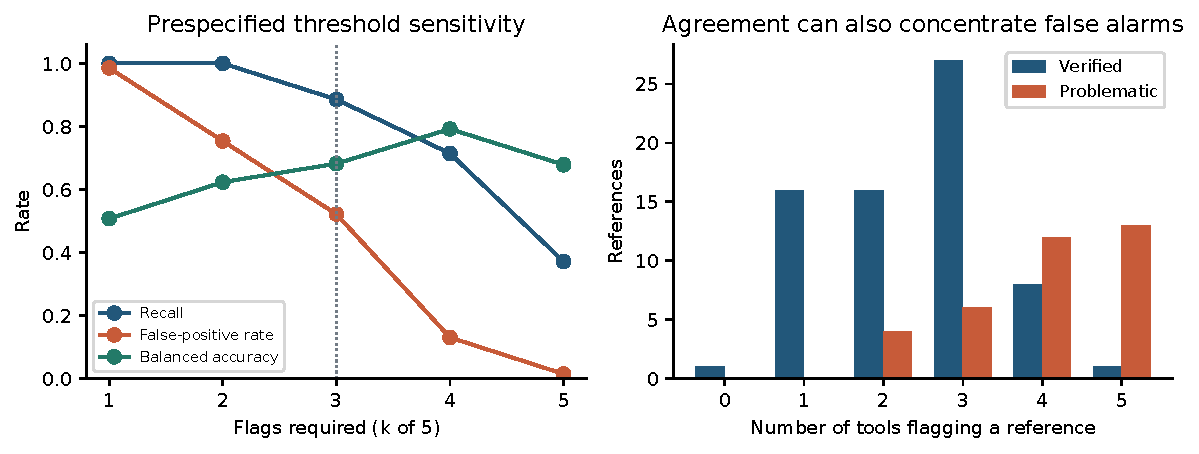
\includegraphics[width=\linewidth]{images/02_thresholds_and_votes.pdf}
\caption{Corrected-label threshold sensitivity and vote-count distribution. At exactly three votes, 27 references are verified and six problematic. Agreement is therefore not sufficient evidence of correctness.}
\Description{A threshold curve shows decreasing recall and false-positive rate, while a grouped bar chart shows the label counts for zero through five flags.}
\label{fig:threshold}
\end{figure}

The vote distribution explains the large change between three and four votes (Figure~\ref{fig:threshold}). Excluding exactly-three-vote cases removes 27 false positives but also six true positives. A strict rule cannot distinguish those cases using the count alone. One verified reference receives five flags, showing that unanimous alerts can still disagree with the released manual label. This is an observed decision pattern, not an independently adjudicated explanation of the underlying bibliographic error.

\subsection{Source-held-out selection}
The adaptive procedure chooses $k=4$ when P1 or P2 is held out, and $k=2$ when P3 is held out (Table~\ref{tab:folds}). Pooled BA is 0.704, below the favorable pooled fixed-$k=4$ value. On P1 and P2, the selected strict threshold detects only one of three and one of four problems, respectively. On P3, the selected permissive threshold catches all 28 problems but flags 26 of 37 verified references.

\begin{table}[tb]
\caption{Source-held-out selection on v1.1.0. Training sizes exclude the held-out document; the duplicate screen excludes zero additional rows.}\label{tab:folds}
\centering\small
\begin{tabular}{@{}lrrrrrr@{}}\toprule
Test source & Train $n$ & Test $n$ & Selected $k$ & Recall & FPR & BA \\
\midrule
P1 & 80 & 24 & 4 & 0.333 & 0.190 & 0.571 \\
P2 & 89 & 15 & 4 & 0.250 & 0.091 & 0.580 \\
P3 & 39 & 65 & 2 & 1.000 & 0.703 & 0.649 \\
\bottomrule\end{tabular}

\end{table}

P3 accounts for 65 of 104 references and 28 of 35 corrected positive labels. Its influence on pooled summaries is consequently substantial. Macro-averaging the three held-out document BAs gives approximately 0.600, whereas the pooled BA is 0.704; the two summaries answer different weighting questions. Figure~\ref{fig:documents} makes the source variation visible. Three folds are too few for a robust estimate of deployment performance, but the exercise exposes a weakness concealed by choosing the best threshold on the pooled corpus.

\begin{figure}[tb]
\centering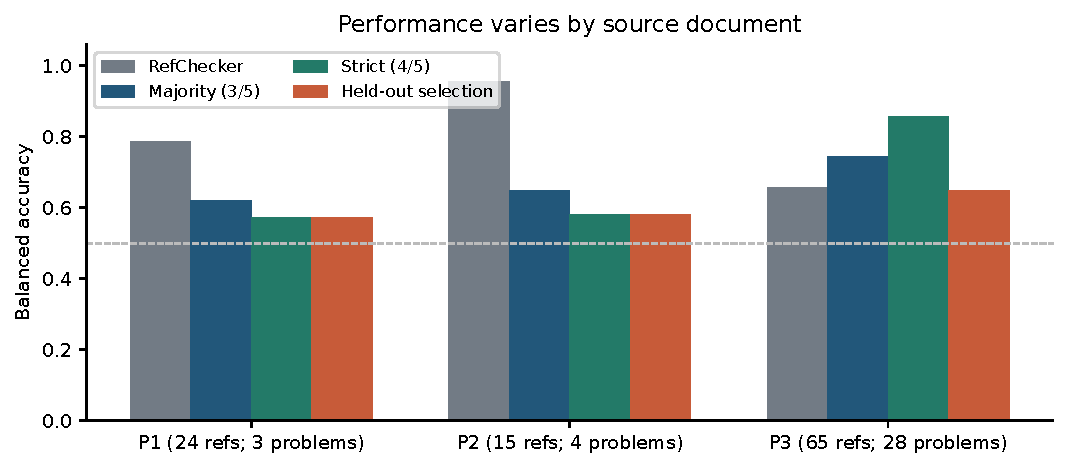
\includegraphics[width=.95\linewidth]{images/03_document_heterogeneity.pdf}
\caption{Corrected-label BA by source document. The fixed four-vote rule performs well on the largest source, while source-held-out threshold selection performs poorly on the two smaller sources.}
\Description{Four methods are compared within P1, P2, and P3, revealing different performance across source documents.}
\label{fig:documents}
\end{figure}

\subsection{Panel ablations and error overlap}
Removing one checker and requiring three of the four remaining flags yields BAs from 0.698 to 0.791. Removing HalRef gives recall 0.800, FPR 0.217, and BA 0.791; removing HalluCiteChecker gives recall 0.886, FPR 0.362, and BA 0.762. Both meet the numerical recall/FPR criterion descriptively on the corrected corpus. These favorable secondary results are reported rather than hidden by the negative primary result. They are not independently validated panel-selection results.

The four-tool rule is more restrictive in vote proportion than the primary three-of-five rule, so the change cannot be attributed only to removal of a weak checker. Selecting the best removal after inspecting the table also introduces selection optimism. A subsequent study would have to select the panel inside the training folds and evaluate it on new sources before recommending it.

Pairwise error-set Jaccard overlaps are exported for all checker pairs. Their presence documents shared mistakes, but overlap alone does not establish statistical dependence or a causal mechanism. The appropriate explanation remains bounded: the observed votes contain enough shared false alerts and minority-only detections to defeat the simple majority objective. Extraction problems, metadata ambiguity, database coverage, and source composition are plausible mechanisms requiring additional evidence.

\subsection{Triage and measured resource scope}
The fixed triage rule accepts 17 references, defers 53, and flags 34. All 17 accepted references are labeled verified. The flagged group contains 25 problematic and nine verified references; the deferred group contains 10 problematic and 43 verified references. Automatic coverage is therefore $51/104=49.0\%$, with nine errors among the automatic decisions. The zero observed false acceptances must not be interpreted as a future safety guarantee.

\begin{figure}[tb]
\centering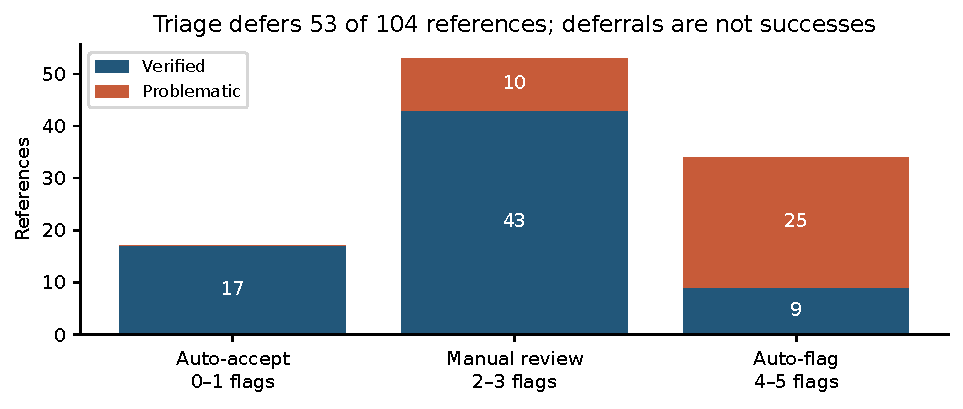
\includegraphics[width=.9\linewidth]{images/06_triage.pdf}
\caption{Corrected-label triage counts. Ten problematic references remain deferred. Conditional recall on automatic cases cannot be reported as overall problem-detection recall.}
\Description{Stacked bars show verified and problematic references in automatic acceptance, manual review, and automatic flagging groups.}
\label{fig:triage}
\end{figure}

Conditional recall among automatically handled problematic cases is 1.0, but that denominator excludes the ten deferred problems. Overall, automatic flags identify only 25 of 35 problematic references. The study measures review-queue size, not human review time, accuracy, or completed adjudication. Seven timing repetitions cover only counting the saved flags for 104 rows. They do not measure the latency or cost of acquiring the five original tool outputs, and no end-to-end efficiency claim is made.

\section{Discussion and Limitations}
The central result is a failure of the chosen simple consensus policy on a specific released corpus. Five opinions do not create five independent pieces of evidence. Majority voting counts decisions without considering what records the tools retrieved, why they disagreed, or whether a flag represents missing information rather than a verified contradiction. The result motivates examining evidence and uncertainty behind alerts instead of treating a vote count as bibliographic truth.

The comparison also separates three different forms of apparent improvement. The pooled four-vote rule improves BA but violates the recall requirement. Two four-tool ablations satisfy the numerical criterion on this sample but have not survived panel-selection validation. The source-held-out selector avoids using each test document's labels to choose its threshold, yet performs weakly and is based on only three sources. Reporting these distinctions prevents a favorable secondary number from becoming an unsupported deployment claim.

Several limitations constrain interpretation. First, the corpus is small and purposively assembled; its positive-label fraction does not estimate citation-error prevalence in the literature. Second, source documents are heterogeneous and clustered. Conditional row bootstrapping cannot compensate for the absence of many independent documents. Third, the original services were not rerun, and binary standardization loses explanations, confidence values, failure states, and service-version details. The results concern released decisions, not the present performance of live tools.

Fourth, manual labels are inherited and were demonstrably revised. The corrected release is preferable for current interpretation, but it does not eliminate annotation uncertainty. Fifth, the duplicate screen is conservative, and differently formatted citations to the same publication could remain. Sixth, the late discovery of v1.1.0 is disclosed rather than recast as a prospective robustness plan. Finally, the experiment measures bibliographic alert agreement; it cannot support conclusions about human trust, formatting effects, semantic claim support, or research misconduct.

Three follow-ups are justified by the findings. The lowest-cost next step is independent adjudication of the disagreement and revised-label cases, with documented evidence and uncertainty. Next, a larger document-diverse corpus would permit nested threshold and panel selection with a genuinely held-out evaluation set. Finally, a version-pinned live-tool rerun could separate retrieval/extraction failures from decision-combination failures. These are proposed studies, not completed experiments in this paper.

\section{Reproducibility and AI Assistance}
The accompanying repository includes raw CC BY 4.0 data with attribution, exact acquisition URLs and hashes, immutable protocol and amendments, source code, sixteen tests, an executed notebook, per-reference predictions, fold memberships, measured CSV tables, bootstrap outputs, and PDF/PNG figures. Tables in this manuscript are generated from the saved results; figures are regenerated by the plotting script. Python and package versions, commands, timestamps, and run manifests identify the execution environment. The data processing is CPU-only and requires no model download or paid API.

Codex assisted with source retrieval, study design, implementation, debugging, execution, analysis, figures, and manuscript drafting. The human requested continuity with prior assignments and rapid completion. The detailed log distinguishes those genuine human instructions from choices made by the assistant. In particular, it does not claim that the student manually reran commands, approved each experimental decision, or completed a live demonstration. Human review of the code, reasoning, and disclosure remains necessary before submission; a prepared walkthrough and viva guide support that review. The record includes actual decoding failures, the label-version correction, and the negative primary outcome.

\section{Conclusion}
On both releases of a 104-reference corpus, fixed majority voting fails to achieve the prespecified reduction in false alarms while retaining the required recall. Corrected labels do not reverse that result. Stricter thresholds and selected panel removals expose potentially useful trade-offs, but pooled improvements do not establish source-level transfer or deployment reliability. The implemented study provides a reproducible way to inspect these trade-offs, preserve negative findings, and distinguish an alert policy from evidence that a citation is correct.

\bibliographystyle{ACM-Reference-Format}
\bibliography{references}
\end{document}
